% Comparative Evaluation of AutoML Frameworks for Tabular Data
% in Resource-Constrained Environments
% 4th Annual Statistics and Data Science Conference 2026 (GSA)
% Tamale Technical University, 25-29 August 2026
%
% Build:  pdflatex automl_presentation.tex  (run twice)
% 15-20 minute slot: ~16 content slides, ~1 minute each.
% Slides marked [UPDATE] contain pilot numbers or placeholders to refresh
% once the full-budget campaign (run_all.sh) has produced final results.

\documentclass[aspectratio=169,10pt]{beamer}

\usetheme{Madrid}
\usecolortheme{seahorse}
\setbeamertemplate{navigation symbols}{}
\setbeamertemplate{caption}{\raggedright\insertcaption\par}

\usepackage{booktabs}
\usepackage{graphicx}
\graphicspath{{../figures/}}

\title[AutoML under Resource Constraints]{Comparative Evaluation of AutoML Frameworks for Tabular Data in Resource-Constrained Environments}
\subtitle{Implications for Data Science Practice in Ghana}
\author[Mumuni \& Ampofo]{Dr.~Hanifatu Napari Mumuni\inst{1} \and Clement Donkor Ampofo\inst{2}}
\institute[TaTU]{\inst{1}Tamale Technical University \and \inst{2}MTech, Data Science}
\date[GSA 2026]{4th Annual Statistics and Data Science Conference \\ Tamale, 25--29 August 2026}

\begin{document}

\begin{frame}
  \titlepage
\end{frame}

\begin{frame}{The question every Ghanaian data team asks}
  \begin{quote}
    \large ``Which ML tool should we actually use, \emph{given what we have}?''
  \end{quote}
  \vfill
  \begin{itemize}
    \item AutoML promises expert-level models without ML engineers
    \item Existing benchmarks assume AWS/GCP or HPC clusters
    \item GSS, Ghana Health Service, MoFA, District Assemblies run on
          \textbf{office-grade laptops and workstations}
    \item No published guidance for that hardware reality
  \end{itemize}
  \vfill
  \textbf{Research question:} which open-source AutoML framework delivers the
  best accuracy-to-resource ratio for tabular tasks on hardware typical of
  Ghanaian public-sector institutions?
\end{frame}

\begin{frame}{Five frameworks under test}
  \centering
  \begin{tabular}{@{}llll@{}}
    \toprule
    Framework & Developer & Claimed strength \\
    \midrule
    AutoGluon    & Amazon AWS       & Highest accuracy, ensemble stacking \\
    PyCaret      & Community        & Fast runs, easy API \\
    FLAML        & Microsoft        & Cost-frugal optimisation \\
    auto-sklearn & AutoML Freiburg  & Competition winner \\
    H2O AutoML   & H2O.ai           & Scalable, fast inference \\
    \bottomrule
  \end{tabular}
  \vfill
  All open-source; all claim to work ``anywhere.''
  We test that claim where it matters.
\end{frame}

\begin{frame}{Three resource tiers, enforced --- not assumed}
  \centering
  \begin{tabular}{@{}lrrrl@{}}
    \toprule
    Tier & RAM & Cores & Budget & Represents \\
    \midrule
    Constrained   & 4\,GB  & 2 & 5\,min  & Basic government office laptop \\
    Moderate      & 8\,GB  & 4 & 15\,min & Institutional workstation \\
    Unconstrained & 16\,GB & 8 & 60\,min & High-spec research machine \\
    \bottomrule
  \end{tabular}
  \vfill
  \begin{itemize}
    \item Docker containers enforce exact RAM/CPU caps per run
    \item A framework that exceeds its container's memory is killed ---
          exactly what happens on a real 4\,GB laptop
    \item Every run independent, seeded (42), logged automatically
  \end{itemize}
\end{frame}

\begin{frame}{Seven datasets spanning public-sector tasks}
  \centering
  \begin{tabular}{@{}llrl@{}}
    \toprule
    Dataset & Task & Rows & Domain \\
    \midrule
    Adult Income        & Binary        & 48\,839  & Finance / policy \\
    Bank Marketing      & Binary        & 41\,188  & Finance \\
    Titanic             & Binary        & 891      & Benchmark standard \\
    Credit Card Fraud   & Binary (0.17\% pos.) & 284\,807 & Risk \\
    California Housing  & Regression    & 20\,640  & Urban planning \\
    Ames Housing        & Regression    & 2\,930   & Urban planning \\
    Wine Quality        & Multiclass    & 6\,497   & Agriculture \\
    \bottomrule
  \end{tabular}
  \vfill
  $5 \text{ frameworks} \times 3 \text{ tiers} \times 7 \text{ datasets}
   = 105$ containerised experimental runs.
\end{frame}

\begin{frame}{What we measure}
  \begin{columns}[t]
    \column{0.48\textwidth}
    \textbf{Predictive quality}
    \begin{itemize}
      \item Weighted F1 (classification)
      \item AUC-ROC (binary)
      \item RMSE (regression)
    \end{itemize}
    \column{0.48\textwidth}
    \textbf{Efficiency \& reliability}
    \begin{itemize}
      \item Training wall-clock time
      \item Peak RAM (whole process tree)
      \item Mean CPU utilisation
      \item \textbf{Completion rate} --- did it finish at all?
    \end{itemize}
  \end{columns}
  \vfill
  Completion rate is the metric high-resource benchmarks never report ---
  and the one that decides whether a tool is usable on a 4\,GB laptop.
\end{frame}

\begin{frame}{Reproducibility as a first-class output}
  \begin{itemize}
    \item Full pipeline open-source: dataset fetch $\to$ container build
          $\to$ 105 runs $\to$ analysis figures, one command per stage
    \item Dataset provenance: source URL + SHA-256 checksum per file
    \item One Docker image per framework (they conflict if co-installed ---
          itself a practical finding)
    \item Every random state seeded at 42
  \end{itemize}
  \vfill
  Any institution can re-run the benchmark on \emph{its own} hardware
  and read off its own recommendation.
\end{frame}

% ---------------------------------------------------------------------------
% RESULTS SECTION -- refresh numbers/figures after the full-budget campaign
% ---------------------------------------------------------------------------

\begin{frame}{[UPDATE] Headline result: the accuracy--memory frontier}
  \centering
  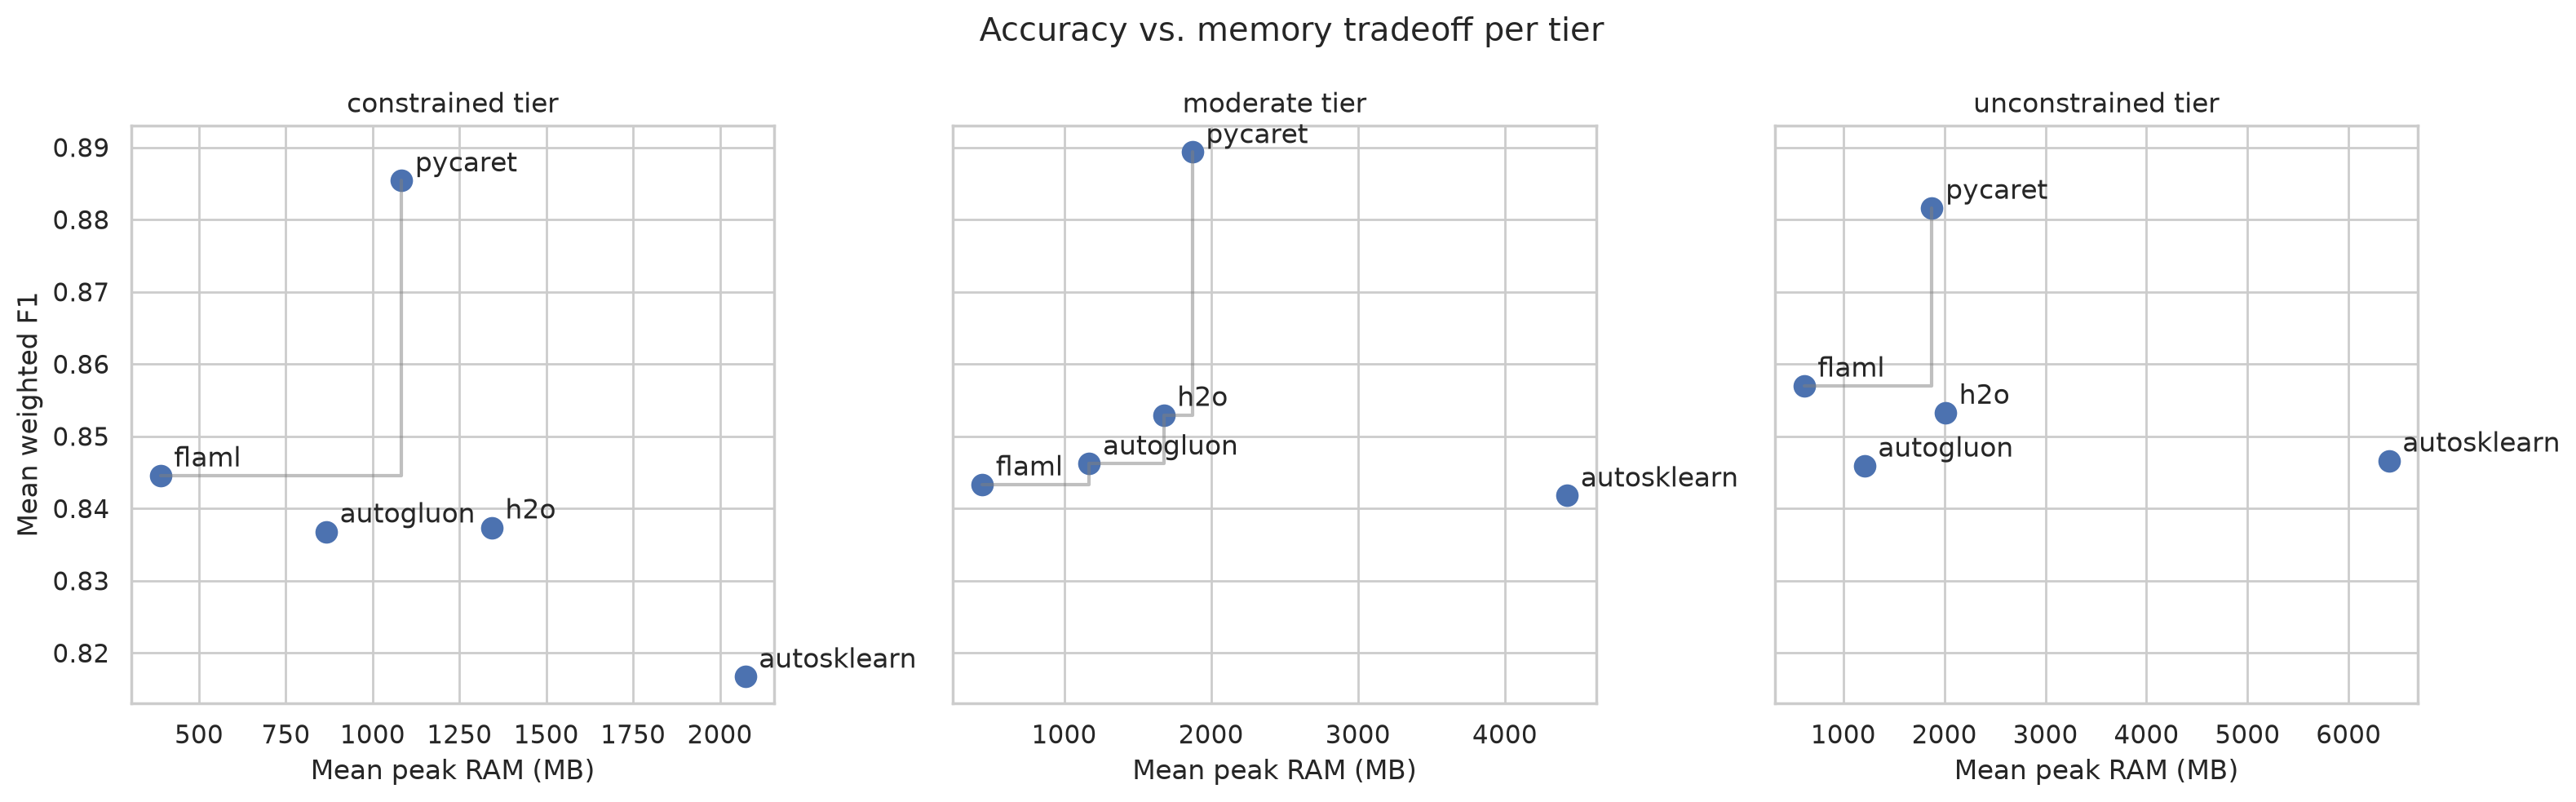
\includegraphics[width=0.9\textwidth,height=0.72\textheight,keepaspectratio]{pareto_plot.png}
  \vfill
  \small One point per framework per tier; up-and-left is better.
\end{frame}

\begin{frame}{[UPDATE] What shrinking resources actually cost}
  \centering
  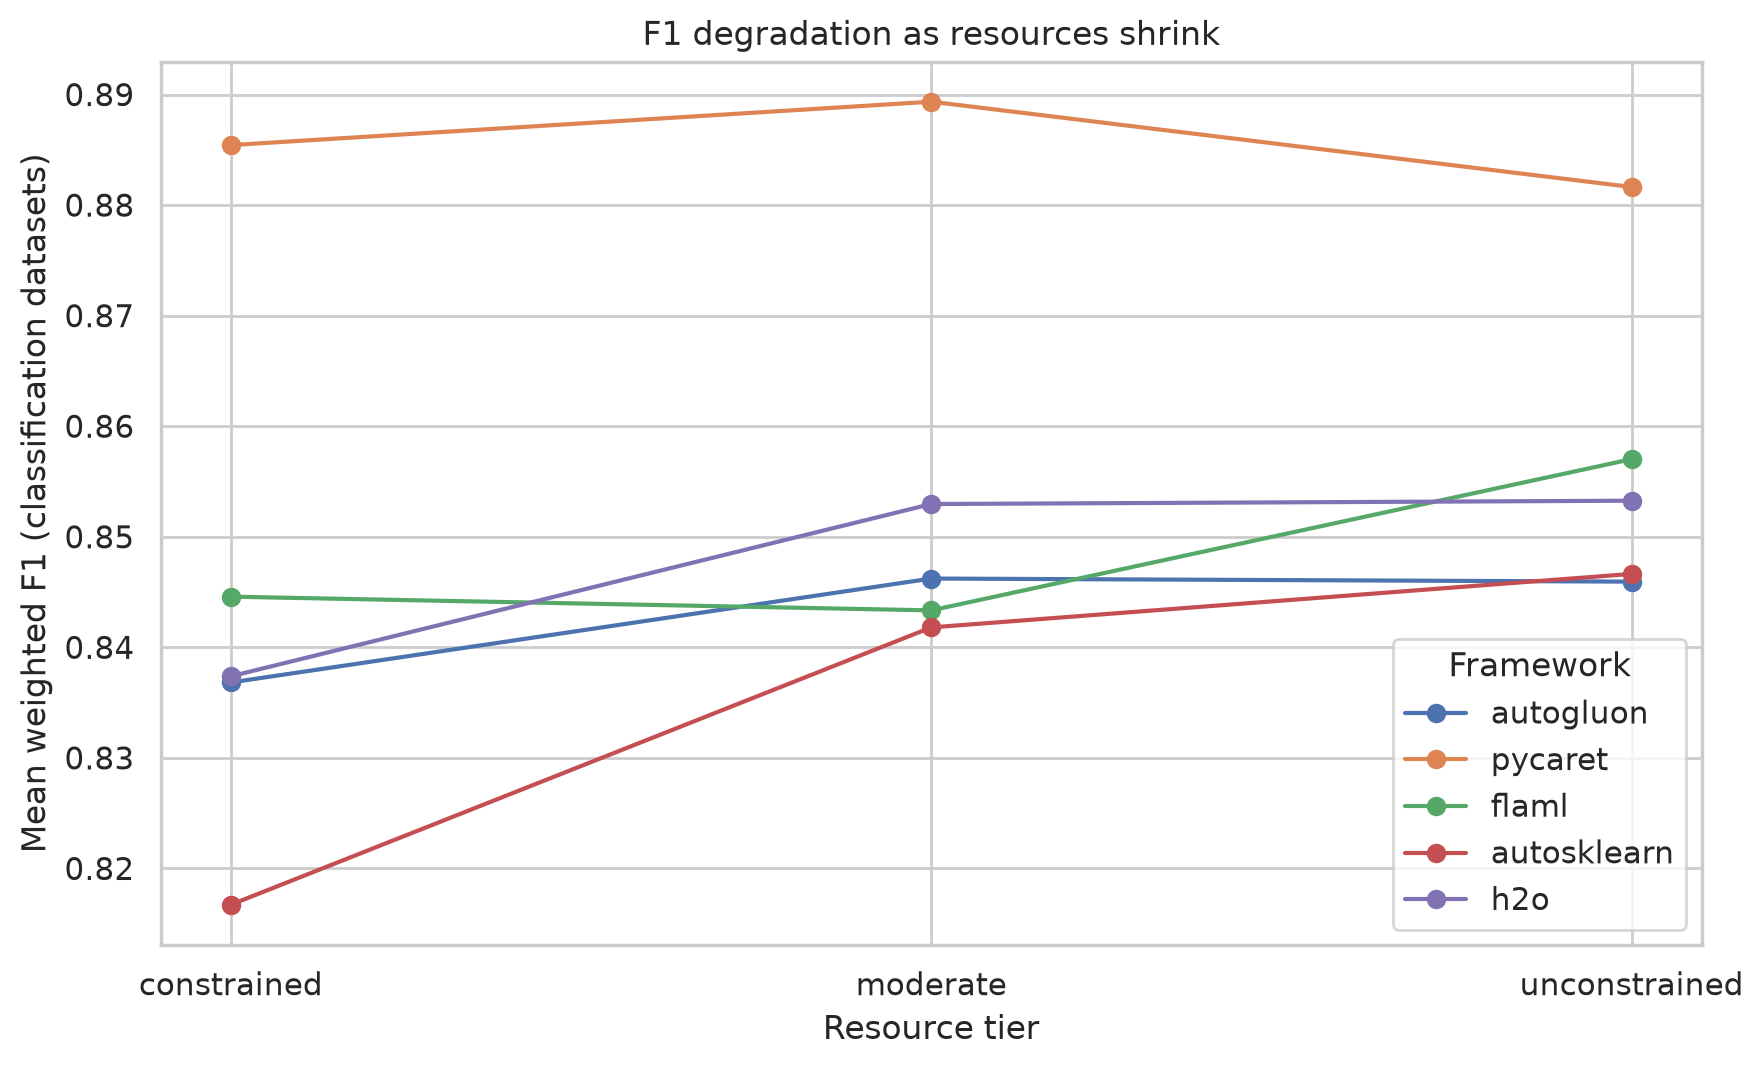
\includegraphics[width=0.9\textwidth,height=0.72\textheight,keepaspectratio]{degradation_curves.png}
  \vfill
  \small Mean weighted F1 per framework as tiers shrink
  (unconstrained $\to$ constrained).
\end{frame}

\begin{frame}{[UPDATE] Who survives the 4\,GB laptop?}
  \centering
  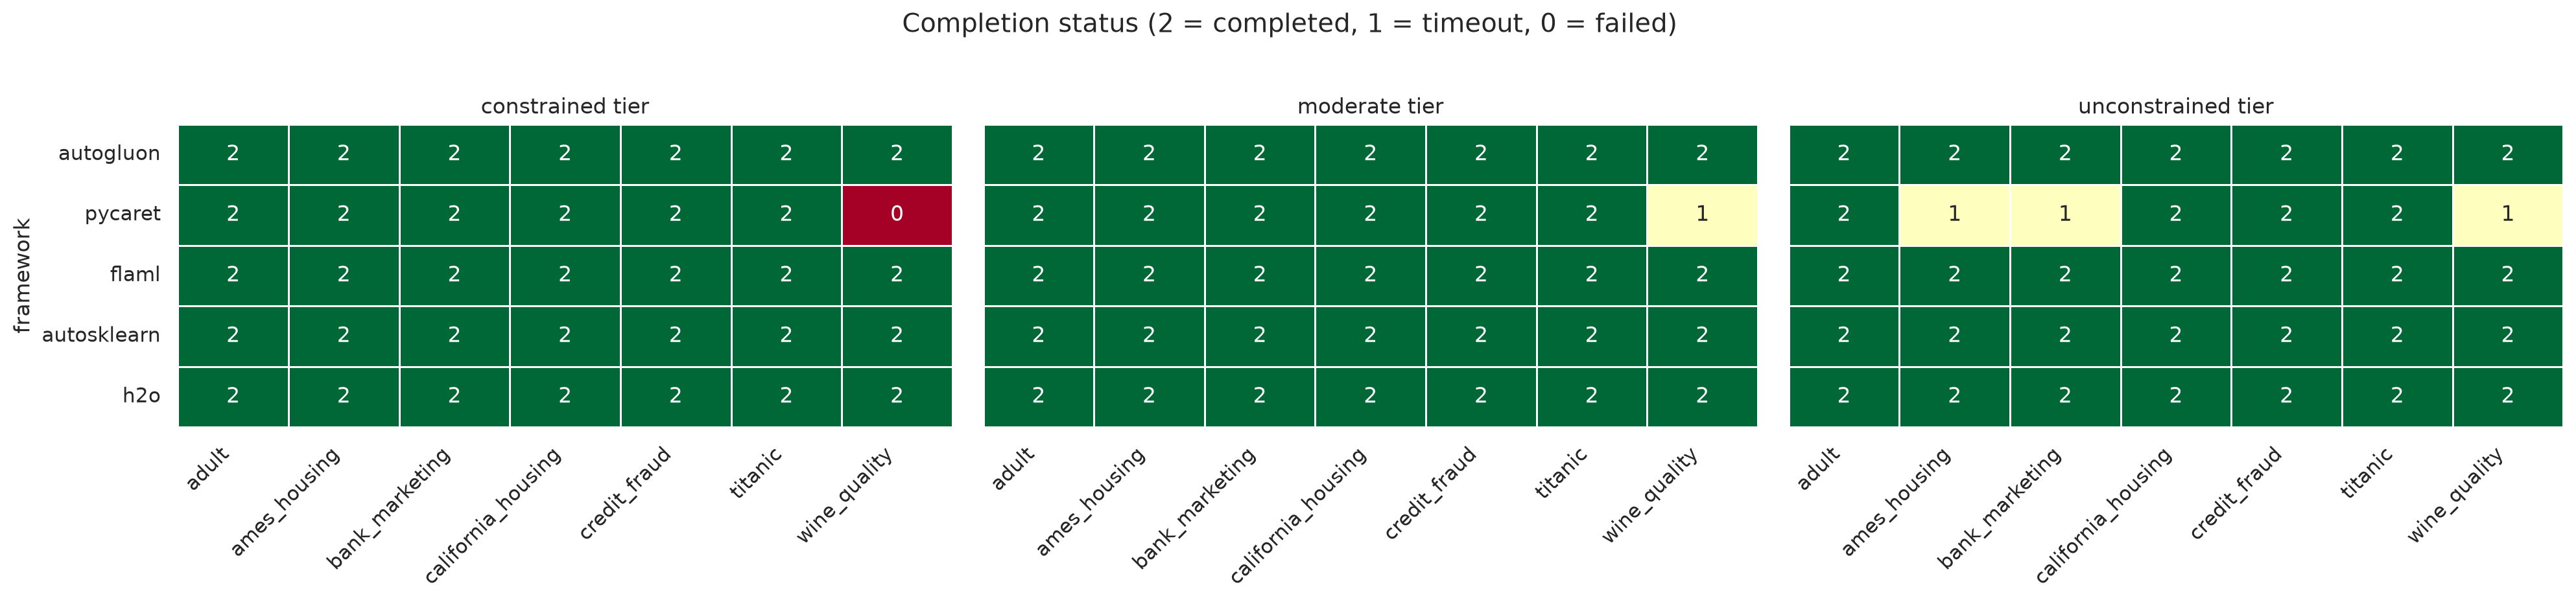
\includegraphics[width=0.9\textwidth,height=0.72\textheight,keepaspectratio]{failure_heatmap.png}
  \vfill
  \small Completion status of all 105 runs
  (2 = completed, 1 = timeout, 0 = failed).
\end{frame}

\begin{frame}{Early findings from the pilot campaign}
  Already visible at reduced budgets (60--240\,s), real datasets, real caps:
  \begin{itemize}
    \item \textbf{Budget discipline differs sharply.} FLAML lands within
          $\pm 2\,\mathrm{s}$ of every budget; PyCaret overran a 120\,s budget
          by $7\times$ on several datasets and had to be externally killed on one
          --- on a shared institutional machine that behaviour matters
    \item \textbf{4\,GB is workable} for lightweight optimisers: the 284\,807-row
          fraud dataset trained to F1 $\approx 0.999$ inside the constrained tier
    \item \textbf{Memory footprints span an order of magnitude} at identical
          accuracy on some tasks (FLAML $\sim$0.3\,GB vs.\ PyCaret $\sim$2\,GB)
    \item Version conflicts between frameworks are real; per-framework
          environments are unavoidable
  \end{itemize}
\end{frame}

\begin{frame}{[UPDATE] Recommendation matrix (draft)}
  \centering
  \begin{tabular}{@{}lll@{}}
    \toprule
    Context & Recommendation & Rationale \\
    \midrule
    4\,GB office laptop        & \emph{[final data pending]} & completion + F1/RAM \\
    8\,GB workstation          & \emph{[final data pending]} & best F1 within caps \\
    16\,GB research machine    & \emph{[final data pending]} & top accuracy \\
    Shared/queued machines     & budget-disciplined tools    & predictable runtimes \\
    Teaching without cloud     & \emph{[final data pending]} & install simplicity \\
    \bottomrule
  \end{tabular}
  \vfill
  The matrix --- not any single score --- is the deliverable institutions
  can act on.
\end{frame}

\begin{frame}{Why this matters for policy and practice}
  \begin{itemize}
    \item \textbf{GSS}: national analytics on standard-issue hardware
    \item \textbf{Ghana Health Service}: predictive analytics in regional
          offices, no cloud dependency
    \item \textbf{MoFA}: crop yield and supply forecasting at district level
    \item \textbf{Universities/polytechnics}: teach AutoML without cloud
          budgets
    \item Procurement guidance: what hardware is \emph{enough}, avoiding
          both under- and over-provisioning
  \end{itemize}
\end{frame}

\begin{frame}{Limitations and future work}
  \begin{itemize}
    \item Tabular data only --- no text, images, or time series
    \item Public benchmark datasets proxy, not replace, Ghanaian
          administrative data
    \item Single-machine focus; no distributed settings
    \item Next: replication on actual institutional hardware with partner
          agencies, and a Ghana-specific dataset suite
  \end{itemize}
\end{frame}

\begin{frame}{Summary}
  \begin{enumerate}
    \item First AutoML benchmark designed around the hardware Ghanaian
          public institutions actually have
    \item 105 containerised runs: 5 frameworks $\times$ 3 enforced resource
          tiers $\times$ 7 datasets
    \item Deliverable: an evidence-based framework selection guide per
          hardware context
    \item Fully open and reproducible --- rerun it on your own machines
  \end{enumerate}
  \vfill
  \centering
  \textbf{Thank you.} \\[1ex]
  \small Dr.~Hanifatu Napari Mumuni --- hmnapari@tatu.edu.gh \\
  Clement Donkor Ampofo --- conference@ghanasa.org
\end{frame}

\end{document}
